% Options for packages loaded elsewhere
\PassOptionsToPackage{unicode}{hyperref}
\PassOptionsToPackage{hyphens}{url}
%
\documentclass[
]{article}
\usepackage{amsmath,amssymb}
\usepackage{lmodern}
\usepackage{ifxetex,ifluatex}
\ifnum 0\ifxetex 1\fi\ifluatex 1\fi=0 % if pdftex
  \usepackage[T1]{fontenc}
  \usepackage[utf8]{inputenc}
  \usepackage{textcomp} % provide euro and other symbols
\else % if luatex or xetex
  \usepackage{unicode-math}
  \defaultfontfeatures{Scale=MatchLowercase}
  \defaultfontfeatures[\rmfamily]{Ligatures=TeX,Scale=1}
\fi
% Use upquote if available, for straight quotes in verbatim environments
\IfFileExists{upquote.sty}{\usepackage{upquote}}{}
\IfFileExists{microtype.sty}{% use microtype if available
  \usepackage[]{microtype}
  \UseMicrotypeSet[protrusion]{basicmath} % disable protrusion for tt fonts
}{}
\makeatletter
\@ifundefined{KOMAClassName}{% if non-KOMA class
  \IfFileExists{parskip.sty}{%
    \usepackage{parskip}
  }{% else
    \setlength{\parindent}{0pt}
    \setlength{\parskip}{6pt plus 2pt minus 1pt}}
}{% if KOMA class
  \KOMAoptions{parskip=half}}
\makeatother
\usepackage{xcolor}
\IfFileExists{xurl.sty}{\usepackage{xurl}}{} % add URL line breaks if available
\IfFileExists{bookmark.sty}{\usepackage{bookmark}}{\usepackage{hyperref}}
\hypersetup{
  pdftitle={Numbers, Complicated},
  hidelinks,
  pdfcreator={LaTeX via pandoc}}
\urlstyle{same} % disable monospaced font for URLs
\usepackage{graphicx}
\makeatletter
\def\maxwidth{\ifdim\Gin@nat@width>\linewidth\linewidth\else\Gin@nat@width\fi}
\def\maxheight{\ifdim\Gin@nat@height>\textheight\textheight\else\Gin@nat@height\fi}
\makeatother
% Scale images if necessary, so that they will not overflow the page
% margins by default, and it is still possible to overwrite the defaults
% using explicit options in \includegraphics[width, height, ...]{}
\setkeys{Gin}{width=\maxwidth,height=\maxheight,keepaspectratio}
% Set default figure placement to htbp
\makeatletter
\def\fps@figure{htbp}
\makeatother
\setlength{\emergencystretch}{3em} % prevent overfull lines
\providecommand{\tightlist}{%
  \setlength{\itemsep}{0pt}\setlength{\parskip}{0pt}}
\setcounter{secnumdepth}{-\maxdimen} % remove section numbering
\ifluatex
  \usepackage{selnolig}  % disable illegal ligatures
\fi

\title{Numbers, Complicated}
\author{}
\date{}

\begin{document}
\maketitle

\textbf{You cannot take the square root of a negative number.} Imagine
you want to find the square root of \(-25\):

\[\sqrt{-25} = \,\, ???\]

It can't be \(-5\), because a negative times a negative is a positive;
negative five times negative five is positive \(25\):

\[(-5)\cdot(-5) = +25\]

It can't be \(+5\), because then where would the negative come from?
\[(+5)\cdot(+5) = +25\] So you cannot take the square root of a negative
number.

So you cannot take the square root of a negative number.

But\ldots{}

\emph{What if you could???}

\textbf{We're about to start talking about complex numbers.} The complex
numbers are what arise when you say, sure, you can take the square root
of a negative number; it's just a new sort of number, which we denote by
\(i\):

\[ \sqrt{-1} = i \]

Any other negative square root we can just write in terms of this
imaginary made-up new number:

\[ \sqrt{-25} = \sqrt{25\cdot(-1)} = \sqrt{25}\cdot\sqrt{-1} = 5\sqrt{-1} = 5i \]

\[ \sqrt{-2} = \sqrt{2\cdot(-1)} = \sqrt{2}\cdot\sqrt{-1} \approx (1.4142\dots )\sqrt{-1} \approx (1.4142\dots )i \]

\[ \text{etc} \]

This is very exciting: the theory of complex numbers rivals calculus as
the most intellectually profound thing we can do in high
school.\footnote{At least, at a \emph{normal} high school, since
  obviously Nueva's math curriculum goes pretty far beyond that!}

You've probably dealt with complex numbers somewhat in Math 2 and
previous classes. We'll start at the beginning anyway. You haven't all
seen exactly the same stuff (or remember all the same stuff), and having
strong foundations is the most important part of building huge
skyscrapers. If you're bored, don't worry---you'll see new stuff soon
enough!

Actually, we won't start totally at the beginning. I don't think we'll
spend too much time justifying the existence of complex numbers, or
motivating them. That's too bad, because the motivation and
justification behind complex numbers is really cool! But it's also way
harder to talk about. (In some sense, the most fundamental things are
often the hardest.\footnote{relatedly:
  \href{https://www.smbc-comics.com/comic/2011-04-04\%5D}{https://www.smbc-comics.com/comic/2011-04-04}}\footnote{``The
  end of all our exploring/will be to arrive where we started/and know
  the place for the first time.''} And I think most of you have done at
least \emph{some} of that in previous years. (Maybe I'll give you some
readings (by other people) or we'll watch a video to that effect.)

Instead, we'll start \emph{in media res}. Is \(\sqrt{-1}\) actually a
valid mathematical object? Does \(\sqrt{-1}\) actually exist?!? For now,
let's just suspend our disbelief. Suspension of disbelief is an
important skill in math as well as in literature. Refusing to read or
disliking \emph{The Lord of the Rings} because hobbits don't exist
misses the point. If the internal logic of a world creates
contradictions, then by all means call them out. Otherwise: live by the
internal logic, suspend your disbelief, and see what you can discover.
That's what we'll do here. We'll act like \(\sqrt{-1}\) is the most
ordinary mathematical object in the world, and just play with it just
like we would any other mathematical object. If the universe ends up
exploding---well, then I guess we'll learn that maybe we shouldn't have
suspended our disbelief. If the universe doesn't appear to
explode---then we've got a brand-new mathematical friend!

So we'll just act all casual about the existence and reality of complex
numbers. Nevertheless, every time you interact with a complex number in
this class, there should still a voice somewhere in the back of your
head screaming, ``IS THIS ALL MADE UP??!! IS THIS ACTUALLY REAL?!?!'' In
fact, that voice in your head should be screaming that not just every
time you use complex numbers, but also every time you use transcendental
numbers (like \(\pi\) or \(e\)), irrational numbers, negative numbers,
zero. How do you know that ANY of those numbers exist or make any sense
as concepts?!? People way, way smarter than you and I spent
\emph{hundreds of years} arguing about those questions.

We must suspend our disbelief---but not fully.

\hypertarget{but-anyway}{%
\subsection{But Anyway}\label{but-anyway}}

Back to suspending our disbelief in the existence and objectivity of
\(i\). Now that we have these new numbers, the complex numbers, we need
to (re-)learn how to do math with them. Namely:

\begin{itemize}
\tightlist
\item
  How do we do \textbf{arithmetic} with complex numbers? We're pretty
  good at arithmetic with real numbers. What about with complex numbers?

  \begin{itemize}
  \tightlist
  \item
    How do we \textbf{add} and \textbf{subtract} complex numbers?
  \item
    How do we \textbf{multiply} and \textbf{divide} complex numbers?
  \item
    How do we takes \textbf{powers} and \textbf{roots} of complex
    numbers?
  \item
    How do we \textbf{exponentiate} and \textbf{logarithm\ldots ate}
    complex numbers?
  \end{itemize}
\end{itemize}

And we know a lot more math than just arithmetic! We'd also like to
learn:

\begin{itemize}
\tightlist
\item
  How do we do \textbf{algebra} with complex numbers? How do
  \textbf{functions} of complex numbers work? What do they look like?
\item
  How do we do \textbf{geometry} with complex numbers?
\item
  How do we do \textbf{calculus} with complex numbers? (Well, I guess we
  should probably learn how to do calculus with real numbers first!)
\end{itemize}

When we generalize and zoom out, things can get weird. We've already
seen this: we played around with polynomials, which were very nice. Then
we generalized to rational functions. Every polynomial is also a
rational function, but there are plenty of rational functions that
aren't polynomials. (Rational functions are what we get if we allow the
exponents to be negative!) And it turns out that if we zoom out to
thinking about all rational functions, things can get pretty weird. We
get asymptotes! (Both the horizontal and vertical kind!)

Similarly, \textbf{do strange new things happen when we zoom out from
the real numbers to the complex numbers?} Which new uncontacted tribes
do we, as mathematical anthropologists, discover and try to understand?
T.S. Eliot writes:

\begin{quote}
Home is where one starts from. As we grow older The world becomes
stranger, the pattern more complicated \ldots{} (\emph{East Coker},
190-191)
\end{quote}

Of course, he wasn't writing about math \emph{per se}, but he might as
well have been, since the poem continues, a few lines later:

\begin{quote}
We must be still and still moving Into another intensity For a further
union, a deeper communion\footnote{ *East Coker*, 204-206} \ldots{}
\end{quote}

Let us move into the intensity of the complex numbers, and in so doing
have a deeper communion with mathematical reality.

\hypertarget{the-first-really-cool-thing-about-i}{%
\subsection{\texorpdfstring{The First Really Cool Thing About
\(i\)}{The First Really Cool Thing About i}}\label{the-first-really-cool-thing-about-i}}

Well, maybe this is the \emph{second} really cool thing about \(i\). The
first cool thing is that it exists at all! (Does it?) But this second
really cool thing about \(i\) is that if we multiply it by itself, a
really cool pattern emerges.

We define \(i\) as the square root of negative one. \emph{But what
happens when we square it}? By definition, squaring a square root
destroys it. Squares and square roots cancel each other out. They're
inverses. So if we multiply \(\sqrt{-1}\) by \(\sqrt{-1}\), we just get
\(-1\). Put more mathematically:

\[
\begin{align*}
i^2 &= i\cdot i \\
&= \sqrt{-1}\cdot \sqrt{-1} \\
&= -1\end{align*}
\]

If this is confusing, think of what happens when we square other square
roots:

\[ \sqrt{5}\cdot\sqrt{5} = 5 \]

\[ \sqrt{374}\cdot\sqrt{374} = 374 \]

\[ \sqrt{2x}\cdot\sqrt{2x} = 2x \]

\[\sqrt{\text{your favorite number}}\,\cdot\,\sqrt{\text{your favorite number}} = \text{your favorite number} \]

So that's what happens when we multiply \(i\) by itself. But what if we
keep going, and keep multiplying the result, and keep raising \(i\) to a
successively higher power?

To start with, does \(i^3\) work out to be anything nice? Well, \(i^3\)
is just \(i^2\) times another \(i\), so this becomes:

\[ 
\begin{align*}
i^3 &= \left(i^2\right)\cdot i \\
&= (-1)\cdot i \\
&= -i
\end{align*}
 \]

What about \(i^4\)? Similar to before, \(i^4\) is just \(i^3\) times
another \(i\), so we have:

\[ 
\begin{align*}
i^4 &= i^3 \cdot i\\
\text{but we just learned that }i^3=-i\text{, so this is:}\\
&= (-i)\cdot i \\
&= -i^2 \\
\text{but we also learned that }i^2=-1\text{, so this is:}\\
&= -(-1)\\
&= +1
\end{align*}
 \]

Let's keep going! How about \(i^5\)? We have:

\[ i^5 = i^4\cdot i = 1\cdot i = i  \]

More! More!

\[ i^6 = i^5 \cdot i = i\cdot i = i^2 = -1  \] We could keep
going---\emph{but it's repeating}! We took \(i\), multiplied it by
itself, and we get this pattern that repeats every four multiplications.
We start with \(i\), then get \(-1\), then \(-i\), then \(1\), then back
to \(i\), then back to \(-1\), and so on and so forth, \emph{ad
infinitum}!

\[ 
\begin{align*}
i^{0} &= +1 \\
i^{1} &= +i \\
i^{2} &= -1 \\
i^{3} &= -i \\
i^{4} &= +1 \\
i^{5} &= +i \\
i^{6} &= -1 \\
i^{7} &= -i \\
i^{8} &= +1 \\
i^{9} &= +i \\
&\vdots
\end{align*}
\]

It's weird, because it's like multiplying something by \(-1\), \emph{but
even more so}. If we multiply things by \(-1\) over and over again, we
get a pattern that repeats every two iterations:

\[(-1)^n = +1, -1, +1, -1, +1, \cdots \]

But if we multiply \(i\) by itself, over and over again, we get a
pattern that repeats \emph{every four iterations}! Wacky. Why
\emph{four}???

I guess if we squint, we can see the powers of \(i\) repeating their
parity (positive/negativeness) every two iterations:

\[ (i)^n = \underbrace{1, i}_{+},\, \underbrace{-1, -i}_{-},\, \underbrace{1, i}_{+},\, \underbrace{-1, -i}_{-},\,  \cdots\]

Likewise, they repeat their one-or-\(i\)-ness every two iterations:

\[ |i^n| = 1,i, 1, i, 1,i, \cdots\]

I guess we can summarize the pattern of powers of \(i\) more concisely:

\[ 
\begin{align*}
i^{(\text{a multiple of }4)} &= +1 \\
i^{(\text{a multiple of }4) \,+\,1} &= +i \\
i^{(\text{a multiple of }4)\,+\,2} &= -1 \\
i^{(\text{a multiple of }4)\,+\,3} &= -i
\end{align*}
\]

This is cool! It's kind of annoying to memorize though---we have to keep
track of whether it's \(1\) or \(i\), and whether it's \(+\) or \(-\).
That's annoying! I wish there were a better way. Is there some
underlying logic to the reason these four elements are in the order
they're in? In other words, why is the pattern this:

\[ \cdots, +i, -1, -i, +1, \cdots\]

And not this:

\[ \cdots, +i,-i,+1,-1, \cdots\quad???\]

or this:

\[ \cdots, +i,+1,-i,-1, \cdots\quad???\]

One answer is ``because that's what we got when we worked out the
algebra,'' but that doesn't seem very \emph{satisfying}. Is there a
better reason? A deeper reason?

This is all \emph{super cool} and I hope it's inspiring us to want to
discover even more about \(i\)! Clearly, \(i\) is a weird number, that
behaves in ways that are unexpected and counterintuitive. Why? What
other weird behaviors do complex numbers have?

\hypertarget{small-print-legalese}{%
\subsection{Small-Print Legalese}\label{small-print-legalese}}

OK, that header is a bit too dismissive. But like with any new
mathematical topic, there's some new vocabulary and notation that we
should quickly get up to speed on. The vocabulary and the notation isn't
the \emph{point}, but it is \emph{antecedent} to the point. When you're
learning how to fly a plane, you need to learn how to adjust the
fuel/oxygen mixture in the engine, and it's not like anyone is
particularly excited about that, or thinks that achieving the perfect
mixture of fuel:oxygen for efficient combustion is why they love flying
planes, but if you get it wrong, the engine stalls and you die.

Here's the first thing to know: \emph{there's nothing imaginary about
the imaginary numbers!} Here's the second thing to know: \emph{there's
nothing complex about the complex numbers!} Imaginary numbers aren't any
more ``imaginary'' than any other numbers (and the ``real'' numbers are
no more or less real than them); complex numbers aren't any more
complicated than non-complex numbers (which are already very complicated
and intricate and beautiful!\footnote{The real numbers AREN'T ACTUALLY
  REAL! None of this is! None of this has material form!}

Gauss supposedly proposed calling imaginary numbers \textbf{lateral
numbers}, deliberately to get rid of the idea that they were
``imaginary'' (or at least more imaginary than real numbers, which he
wanted to call \textbf{direct numbers}). I really like that, because it
removes the value judgments slash other connotations associated with our
vernacular definitions of ``real,'' ``complex,'' and ``imaginary.''

An \textbf{imaginary number} is a multiple of \(i\), that is, a multiple
of \(\sqrt{-1}\). Here are some imaginary numbers:

\[\text{examples of imaginary numbers: } i,\, 5i,\, -2i,\, \pi i,\, \frac{i}{12}\]

A \textbf{complex number} is a twofer: a hybrid chimera with one
real-numbered parent and one imaginary-numbered parent. It consists of
two real numbers added together, with the second one multiplied by
\(i\). So any complex number \(z\) we can write as:

\[z = a + bi\]

where \(a\) and \(b\) are both real numbers. \(a\) is the \textbf{real
component} (or the \textbf{real part}) and \(b\) is the
\textbf{imaginary component} (or the \textbf{imaginary part}). Note that
\(b\) is itself a real number---it's the \emph{coefficient} on the \(i\)
term, but it doesn't include the \(i\) itself. Here's another way to put
that:

\[\text{a complex number} = (\underbrace{\text{a real number}}_{\text{real component}}) + (\underbrace{\text{another real number}}_{\text{imaginary component}})\cdot \underbrace{i}_{i}\]

As a practical matter, we tend to use the variables \(z\) and \(w\) to
denote complex numbers (and \(x\) and \(y\) to denote real
numbers)\footnote{Sometimes I think we should take more inspiration from functional programming and strongly-typed programming languages, and be more explicit about the types of our variables, and in lots of more formal math textbooks people do just that, but oh well.}.

Here's an observation: \emph{every real number is also a complex
number}. It's just that real numbers have imaginary part of \(0\). For
example, we can think of the real number \(5\) as being also a complex
number: it's \(5+0i\). It has real part \(5\), and imaginary part \(0\).
This is like how every integer is \emph{also} a rational number: \(7\)
is a rational number, because we can write it as the ratio of two
integers, \(7/1\).

Likewise, every imaginary number is also a complex number: we can think
of the imaginary number \(7i\) as being \(0+7i\), so it has real part
\(0\) and imaginary part \(7\).

Here are some more examples of numbers and where they fit in our
typology/cladogram of numbers:

\begin{itemize}
\tightlist
\item
  \(5\) is a real number. It's also a complex number. It's not an
  imaginary number.
\item
  \(i\) is a complex number. It's also an imaginary number. It's not a
  real number.
\item
  \(2+7i\) is a complex number. It's neither real nor imaginary.
\item
  \(12i\) is a complex number. It's also an imaginary number. It's
  definitely not a real number.
\end{itemize}

And here's a Venn diagram---well, more like an ordinary set-containment
diagram---of how the complex numbers relate to the real and imaginary
numbers (and whatever even larger classes of numbers there might be):

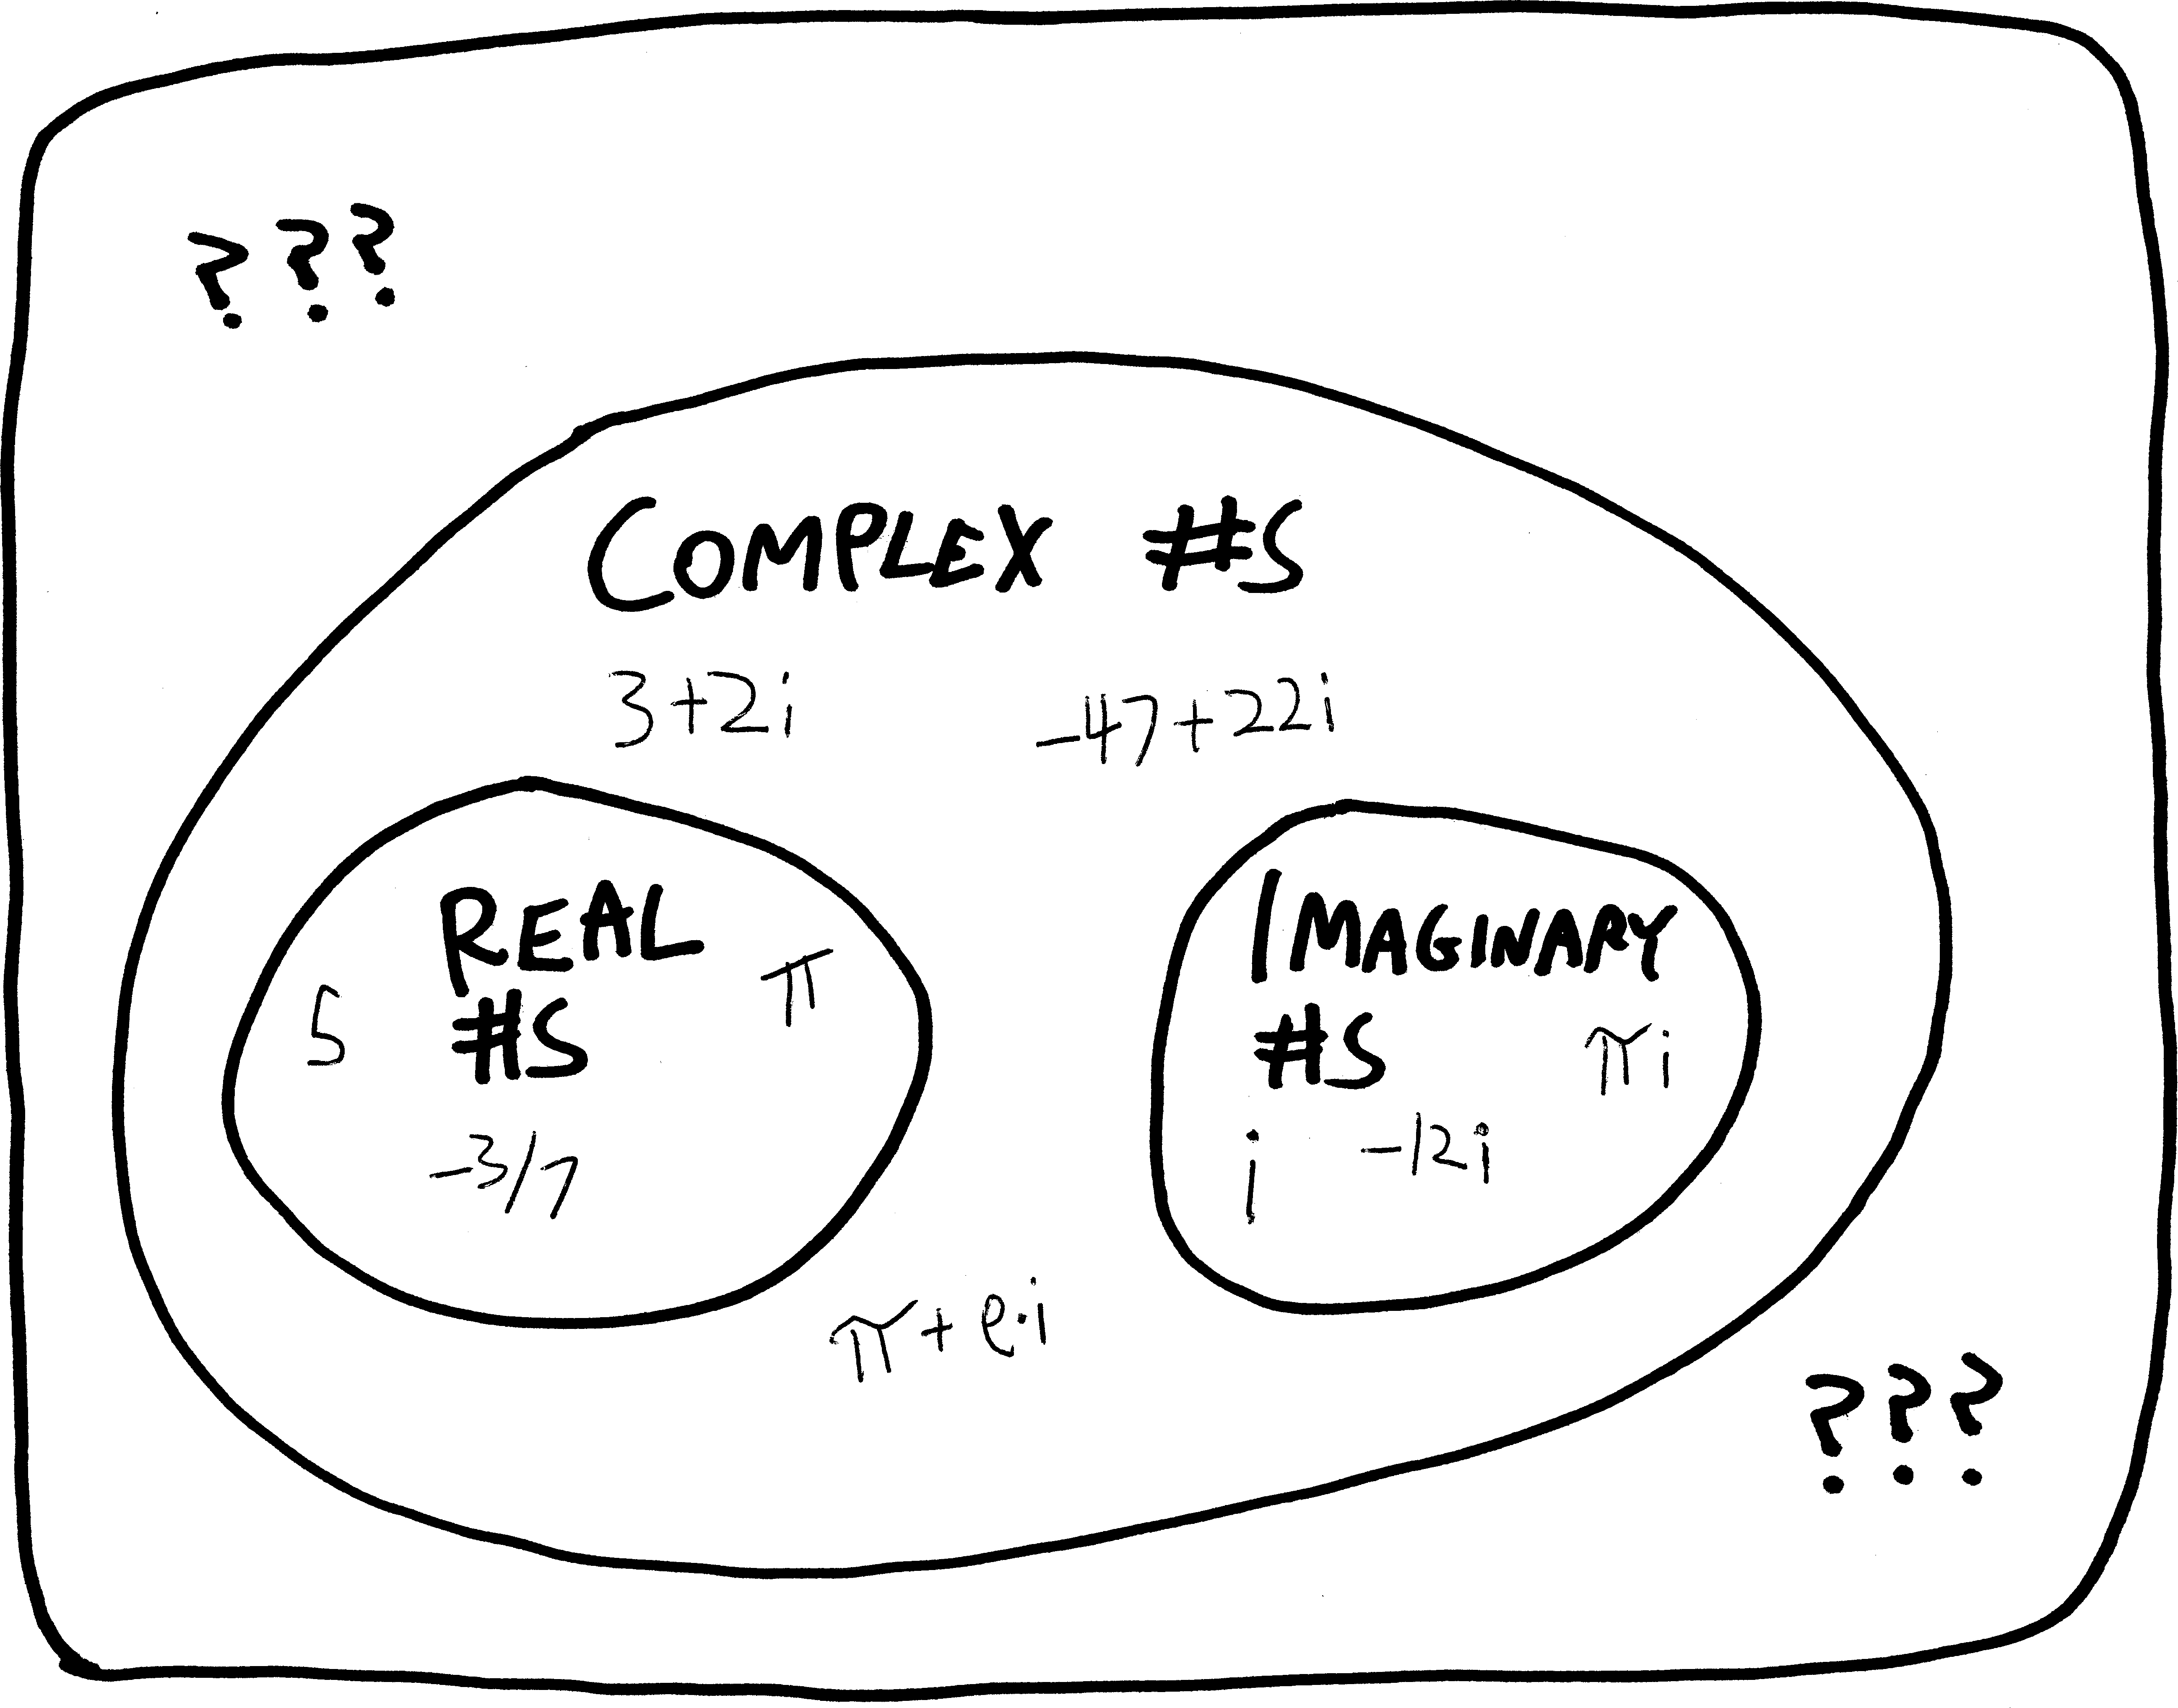
\includegraphics{./complex-numbers-set-diagram.png}

Often if we just want to talk about the real part or the imaginary part
of a number, we'll describe it with function notation:

\[Re(z) = \text{the real part of } z\]

\[Im(z) = \text{the imaginary part of } z\]

So, for example:

\[Re(2+7i) = 2\]

\[Im(2+7i) = 7\]

Note that \(Im(2+7i)\) is \emph{not} \(7i\)! It's just \(7\). The
imaginary part is only the \emph{coefficient} on the \(i\) part.

Somewhat more generally, we can write:

\[Re(a+bi) = a\]

\[Im(a+bi) = b\]

Question: can we come up with a formula that takes in a complex number
and churns out the real and/or imaginary parts? Like, something more
algebraic? Something somewhat more mathematically sophisticated than
just pointing to the real or imaginary component and saying ``it's that
thing!''

\hypertarget{adding}{%
\subsection{Adding}\label{adding}}

We can add two complex numbers together to get a \emph{third} complex
numbers! All we do is add the real part, and add the imaginary part! The
two parts stay totally seperate from each other! So, for example:

\[
\begin{align*}
(5+2i)\,+\,(3+7i) &= (5+3) \,+\,(2+7)i \\
&= 8 + 9i
\end{align*}
\]

\hypertarget{subtracting}{%
\subsection{Subtracting}\label{subtracting}}

We can subtract complex numbers, too.

\hypertarget{multiplying}{%
\subsection{Multiplying}\label{multiplying}}

We can multiply complex numbers! But it's \emph{not} quite as simple as
addition and subtraction. We \emph{don't} independently multiply the
real and complex parts:

\[(5+2i)\cdot(3+7i) \,\neq\, (5\cdot3) + (2\cdot7)i\]

Adding complex numbers is easy, because a complex number is just two
real numbers added, and so things play together nicely. But when we try
to multiply a complex number, then all of a sudden we're combining
\emph{multiplication} with \emph{addition}! So we need to think about
how those two operations interact. They interact via our old friend, the
distributive property:

\[a(b+c) = ab + ac\]

So to multiply two complex numbers, we do the same thing as we would to
multiply any other binomial. We can use the distributive law or FOIL it
or what-have-you. So, for example:

\[
\begin{align*}(3+2i)(5+7i) &= 3\cdot 5 \,+\, 3\cdot7i\,+\,3\cdot2i + 2i\cdot7i \quad \text{(by FOIL or whathaveyou)} \\
&= 15 + 30i + 14i^2 \quad \text{(combining terms)} \\
\text{But wait! $i^2=-1$, so this becomes:}\\
&= 15 + 30i + 14\cdot(-1) \\
&= 1 + 30i
\end{align*}
\]

If we wanted to make a formula into which we could plug any two complex
numbers, we could just take two arbitrary complex numbers, multiply them
together, and see what happens. By ``arbitrary'' I mean that we could
take two complex numbers \emph{that in fact stand in for all complex
numbers}. In other words, we could have \(a+bi\) as one complex number,
where \(a\) and \(b\) could be any real number, and we could have
\(c+di\), where \(c\) and \(d\) could be any real number. What happens
when we multiply them togther?

\[
\begin{align*}(a+bi)(c+di) &= a\cdot c \,+\, a\cdot di\,+\,c\cdot bi + bdi^2 \\
&= ac + (ad + cb)i + bdi^2  \\
&= ac + (ad + cb)i + bd\cdot(-1) \\
&= \underbrace{(ac-bd)}_{\text{real part}} \,+\,  \underbrace{(ad + cb)}_{\text{imaginary part}}\cdot i
\end{align*}
\]

I guess you could memorize this formula if you want to, but there's no
point---since you're already comfortable and familiar with multiplying
out binomials, you should probably just do the same thing you do there
(FOIL it or distribute it or whatever). Of course, if you were going to
write a computer program that dealt with complex numbers, you'd probably
want to write in a formula like this.

\hypertarget{dividing}{%
\subsection{Dividing}\label{dividing}}

Division is trickiest. Suppose we want to divide two complex numbers,
\(2+3i\) and \(5+7i\):

\[\frac{2+3i}{5+7i}\]

Our first question here ought be: is it going to be another complex
number, or some more weird and esoteric type of number?? More generally,
when we divide two complex numbers, do we always a complex number? If we
divide integers, we don't always get another integer----e.g., \(5/7\) is
a rational number, not an integer. Of all our four basic arithmetic
operations, division is the scariest, and the hardest. We do long
division, but we don't do ``long addition.'' Division is sometimes
wormholes us out to extra dimensions of numbers. We take two nice,
clean, well-behaved integers like \(5\) and \(7\), divide them, and we
get a horrible non-integer:

\[\text{two nice integers} \rightarrow\quad \frac{5}{7} \,=\, \underbrace{0.714285714285714285714285714285714285714285714285714285714\dots\dots}_{\text{terrifying thing that's definitely not an integer}}\]

So, if we divide two complex numbers, what happens?

We'll answer that broader question in a minute. But first, back to
dividing these two specific complex numbers. \emph{If} their quotient
does indeed turn out to be another complex number, \emph{then} we should
be able to write it in \(a+bi\) form. We should be able to figure out
what both the real and imaginary parts are. In other words, we should
end up with:

\[\frac{2+3i}{5+7i} = (\underbrace{\text{something}}_{\text{the real part}}) + (\underbrace{\text{something else}}_{\text{the imaginary part}})\cdot i\]

But how do we actually figure out what those parts are? Fractions are
hard. Division is messy (even with real numbers and variables.)

Somehow, we need to bribe, bully, convince, or cajole our quotient to
get into that form. The problem is that we've got two separate things on
the bottom, \(5\) and \(7i\). So we can't just cleanly split the
fraction up along those two things. Many of you were trying to do just
that last semester, and it made me quite sad:

\[\frac{a}{b+c} \neq \frac{a}{b} + \frac{a}{c}\]

However, \emph{if} we could somehow turn the two things on the bottom
into \emph{one} thing, we'd be set, because then we *can\} split the
tops up:

\[\frac{(\text{something})+(\text{something else})\cdot i}{\text{one thing}} \,=\, \frac{\text{something}}{\text{one thing}} + \frac{\text{something else}}{\text{one thing}}\cdot i\]

So if we could do that, then we'd have a complex number, in standard
\((\text{real part})+(\text{imaginary part})\cdot i\) form. So, how can
we do that? Can we get the \(i\) out of the denominator, so that we only
have a real number on the bottom?

Here's the idea: what if we multiply the denominator by itself, but not
\emph{quite} by itself. Let's change the sign between the real part and
the imaginary part, from \(+5i\) to \(-5i\). If we do that, what
happens?

\[
\begin{align*}
(5+7i)\cdot(5-7i) &= 5\cdot5 \,+\, 5\cdot7i \,-\, 5\cdot7i \,-\, (7i)^2 \\
&= 25 \,\,\, \cancel{+\, 5\cdot7i} \,\,\, \cancel{-\,5\cdot7i} \,-\, 7^2i^2 \\
&= 25- 49\cdot(-1) \\
&= 74
\end{align*}
\]

The \(i\) goes away!!!! The two \(i\) terms cancel each other out! We
get an \(i^2\) term, sure, but \(i^2\) is just \(-1\), so that turns
into an ordinary real number, too. No \(i\)s!!!

So if we multiply the bottom of this fraction by this thing, we'd get
rid of the \(i\):

\[\frac{2+3i}{5+7i}\cdot \frac{}{5-7i} = \frac{}{74}\]

There's a major catch: we can't go willy-nilly multiplying random parts
of our expression by random other numbers. That's not licit. We can't do
that. It'd turn into something totally different. So if we want to
multiply the bottom of the expression by \(5-7i\), then we need to
multiply the top by \(5-7i\), too, so that we're not actually changing
anything. Instead, we're just multiplying it by \(1\)---a weird form of
\(1\), but \(1\) nonetheless.

\[\frac{(2+3i)}{(5+7i)}\cdot\underbrace{\frac{(5-7i)}{(5-7i)}}_{=1}\]

So, there's a cool trick! What if we try multiplying this thing by
\(1\)---but by a very special form of \(1\):

\[\frac{(2+3i)}{(5+7i)}\cdot\underbrace{\frac{(5-7i)}{(5-7i)}}_{=1}\]

Anything over itself is equal to \(1\), and we can multiply anything by
\(1\) without changing it. We're not violating any laws of algebra.
We've found this special form of \(1\) by taking the denominator, and
flipping the sign on the imaginary part (i.e., going from \(5+7i\) to
\(5-7i\)), and then putting that over itself.

Anyway, let's do the full division, and see what happens:

\[
\begin{align*}
\frac{(2+3i)}{(5+7i)}\cdot\frac{(5-7i)}{(5-7i)} &= \frac{2\cdot5 \,-\, 2\cdot7i \,+\, 5\cdot3i \,-\, 3i\cdot7i}{5\cdot5 \,\underbrace{-\, 5\cdot7i \,+\, 5\cdot7i}_{=0} \,-\, 7i\cdot7i} & \text{(just FOIL'ing)} \\ \\
&= \frac{10+i-21i^2}{5\cdot5 \,\underbrace{-\, 5\cdot7i \,+\, 5\cdot7i}_{=0} \,-\, 7i\cdot7i} & \text{(combining terms on the top)} \\ \\
&= \frac{10+i-21i^2}{5\cdot5 \,-\, 7i\cdot7i} & \text{(the $i$ terms cancel out on the bottom!)} \\ \\
&= \frac{10+i-21i^2}{25 \,-\, 49i^2} & \\ \\
&= \frac{10+i+21}{25 + 49} & (i^2=-1)\\ \\
&= \frac{31+i}{74} & \text{(combining terms)}\\ \\
&= \frac{31}{74} + \frac{i}{74} &\text{(separating into real and imaginary components)}\\ \\
&= \frac{31}{74} + \frac{1}{74}i
\end{align*}
\]

If we multiply by that very special form of \(1\), the \(i\) terms
cancel out on the bottom, and we get just a single real term on the
bottom! Then we can split up the fraction, and we can write the quotient
as a genuine complex number, with the real and imaginary parts clear and
obvious and isolated:

\[\frac{(2+3i)}{(5+7i)}= \frac{31}{74} + \frac{1}{74}i\]

What was that special form of \(1\) that we multiplied by? It's called
the \textbf{conjugate} (or the \textbf{complex conjugate}). For any
given complex number \(a+bi\), its conjugate is \(a-bi\). We often
denote it by writing \(\text{Conj}(z)\), or putting a little
\(\overline{\text{flat hat}}\) on top of the number, or superscripting
an asterisk, like \(z^*\). It's pronounced ``{[}zee{]} conjugate'' or
``{[}zee{]}
star.''\footnote{Unless you're my Canadian grandfather, in which case it's "[zed] conjugate'' or "[zed] star."}
More formally,

\[\text{ if } z=a+bi,\quad \text{ then $\quad$ Conj}(z)=\overline{z} = z^*= a-bi\]

We've seen conjugates before; we just haven't used that name for them.
Suppose we're multiplying together two binomials which are identical
except for their signs:

\[(a+b)(a-b)\]

The cool thing that happens is that the cross terms (i.e.~the \(ab\)
terms) cancel out and disappear!

\[
\begin{align*}
(a+b)(a-b) &= a^2 + ab - ab -b^2 \\
&= a^2 - b^2
\end{align*}
\]

And we're left with just powers of \(a\) and \(b\). So if we do this
with a complex number written as a binomial (i.e., \(a+bi\)), the \(i\)
terms disappear, and we're left with just real terms and \(i^2\) terms,
and since \(i^2=-1\), we're left in fact with ONLY real terms:

\[
\begin{align*}
(a+bi)(a-bi) &= a^2 +abi - abi -b^2i^2 \\
&= a^2 -b^2(-1) \\
&= a^2+b^2
\end{align*}
\]

Hey! You know, this also shows us something ELSE that's kind of cool. We
multiply these two complex numbers together, \emph{and we get a real
number}:

\[\underbrace{(a+bi)(a-bi)}_{\text{complex numbers}} = \underbrace{a^2+b^2}_{\text{a real number}}\]

That's exactly the point---we made up this ``conjugate'' thing
specifically as a way of getting rid of \(i\). But still, it's a little
weird, because it's like we're putting together these two complicated
objects, and the object we get as a result isn't an equally-complicated
object (or a \emph{more} complicated object); it's a \emph{simpler}
object.

That's\ldots{} a little weird? I mean, I guess it's something we've seen
before. We can multiply two rational numbers and get an integer:

\[\frac{6}{5}\cdot\frac{10}{6} = 2\]

But still, it's like, we're putting together these two complicated
objects, and the object we get as a result isn't an equally-complicated
object (or a \emph{more} complicated object); it's a \emph{simpler}
object.

The contrasting example, I guess, is with division: we can divide two
integers, and potentially get a number that's not an integer:

\[\frac{3}{5} = \text{not an integer}\]

So in that case, we take two simple objects, combine them, and get a
more-complicated object.

Anyway, so we've found that if we divide \(2+3i\) by \(5+7i\), we get
another complex number, \(\frac{31}{74} + \frac{1}{74}i\). But that
still leaves us with the broader question: if we divide two complex
numbers, do we \emph{always} get another complex number? Or do we
sometimes get a scarier and more exotic form of number? When we divide
two integers, \emph{sometimes} we get a scary non-integer, but not
\emph{always}. Sometimes we divide two nice integers, and we get another
nice integer:

\[\text{two integers} \rightarrow\quad \frac{10}{2} = 5 \quad \longleftarrow\text{another integer}\]

Division, then, is like a dog with aggression problems. Sometimes it
acts cute---but other times it tears your face off. You're never totally
sure which you're going to get. So even when it's being cute, you can
never \emph{fully} trust it. Likewise here. Can we ever fully trust
division of complex numbers? (You'll work out the answer in one of the
homework problems.)

Anyway, the main point to take away from this very long and rambling
section is this: \textbf{if we want to divide two complex numbers, we
can multiply by the conjugate of the denominator (over itself)} to then
be able to figure out the resulting complex number (cleanly).

\medskip
\centerline{
\fbox{
  \parbox{5.5in}{ \medskip\centerline**  Dividing complex numbers, in summary:}
$$\underbrace{\frac{a+bi}{c+di}}_{\substack{\text{trying to }\\\text{divide these}}}\cdot\underbrace{\frac{c-di}{c-di}}_{\substack{\text{multiplying by the}\\\text{ conj. of the denom.}\\\text{over itself, i.e. $1$}}} \quad=\quad  (\underbrace{\text{something}}_{\text{the real part}}) \,+\, (\underbrace{\text{something else}}_{\text{the imaginary part}})\cdot i$$
}
}

\} \medskip

(This still seems kind of messy! If only there were an easier way\ldots)

\hypertarget{graphing-complex-numbers}{%
\subsection{Graphing Complex Numbers}\label{graphing-complex-numbers}}

One way we can think about the real numbers visually is to graph them on
a number line! It's not all that interesting---real numbers are
one-dimensional, so they're just points on a line. (\emph{Functions} of
real numbers is where things start to get interesting, because then
we've got two dimensions---one for the input, one for the output---and
we can start having pretty shapes.)

Complex numbers, on the other hand, \emph{are two dimensional}. In our
construction of them, each complex number is the \emph{unified fusion of
two real numbers}. So if we want to think about complex numbers
visually, we need \emph{two} dimensions---one for each number. Usually
we do this by plotting the real component along the horizontal axis (or
the \textbf{real axis}), and the imaginary component along the vertical
axis (or \textbf{imaginary axis}).

Here are a few examples of complex numbers plotted on the complex plane:

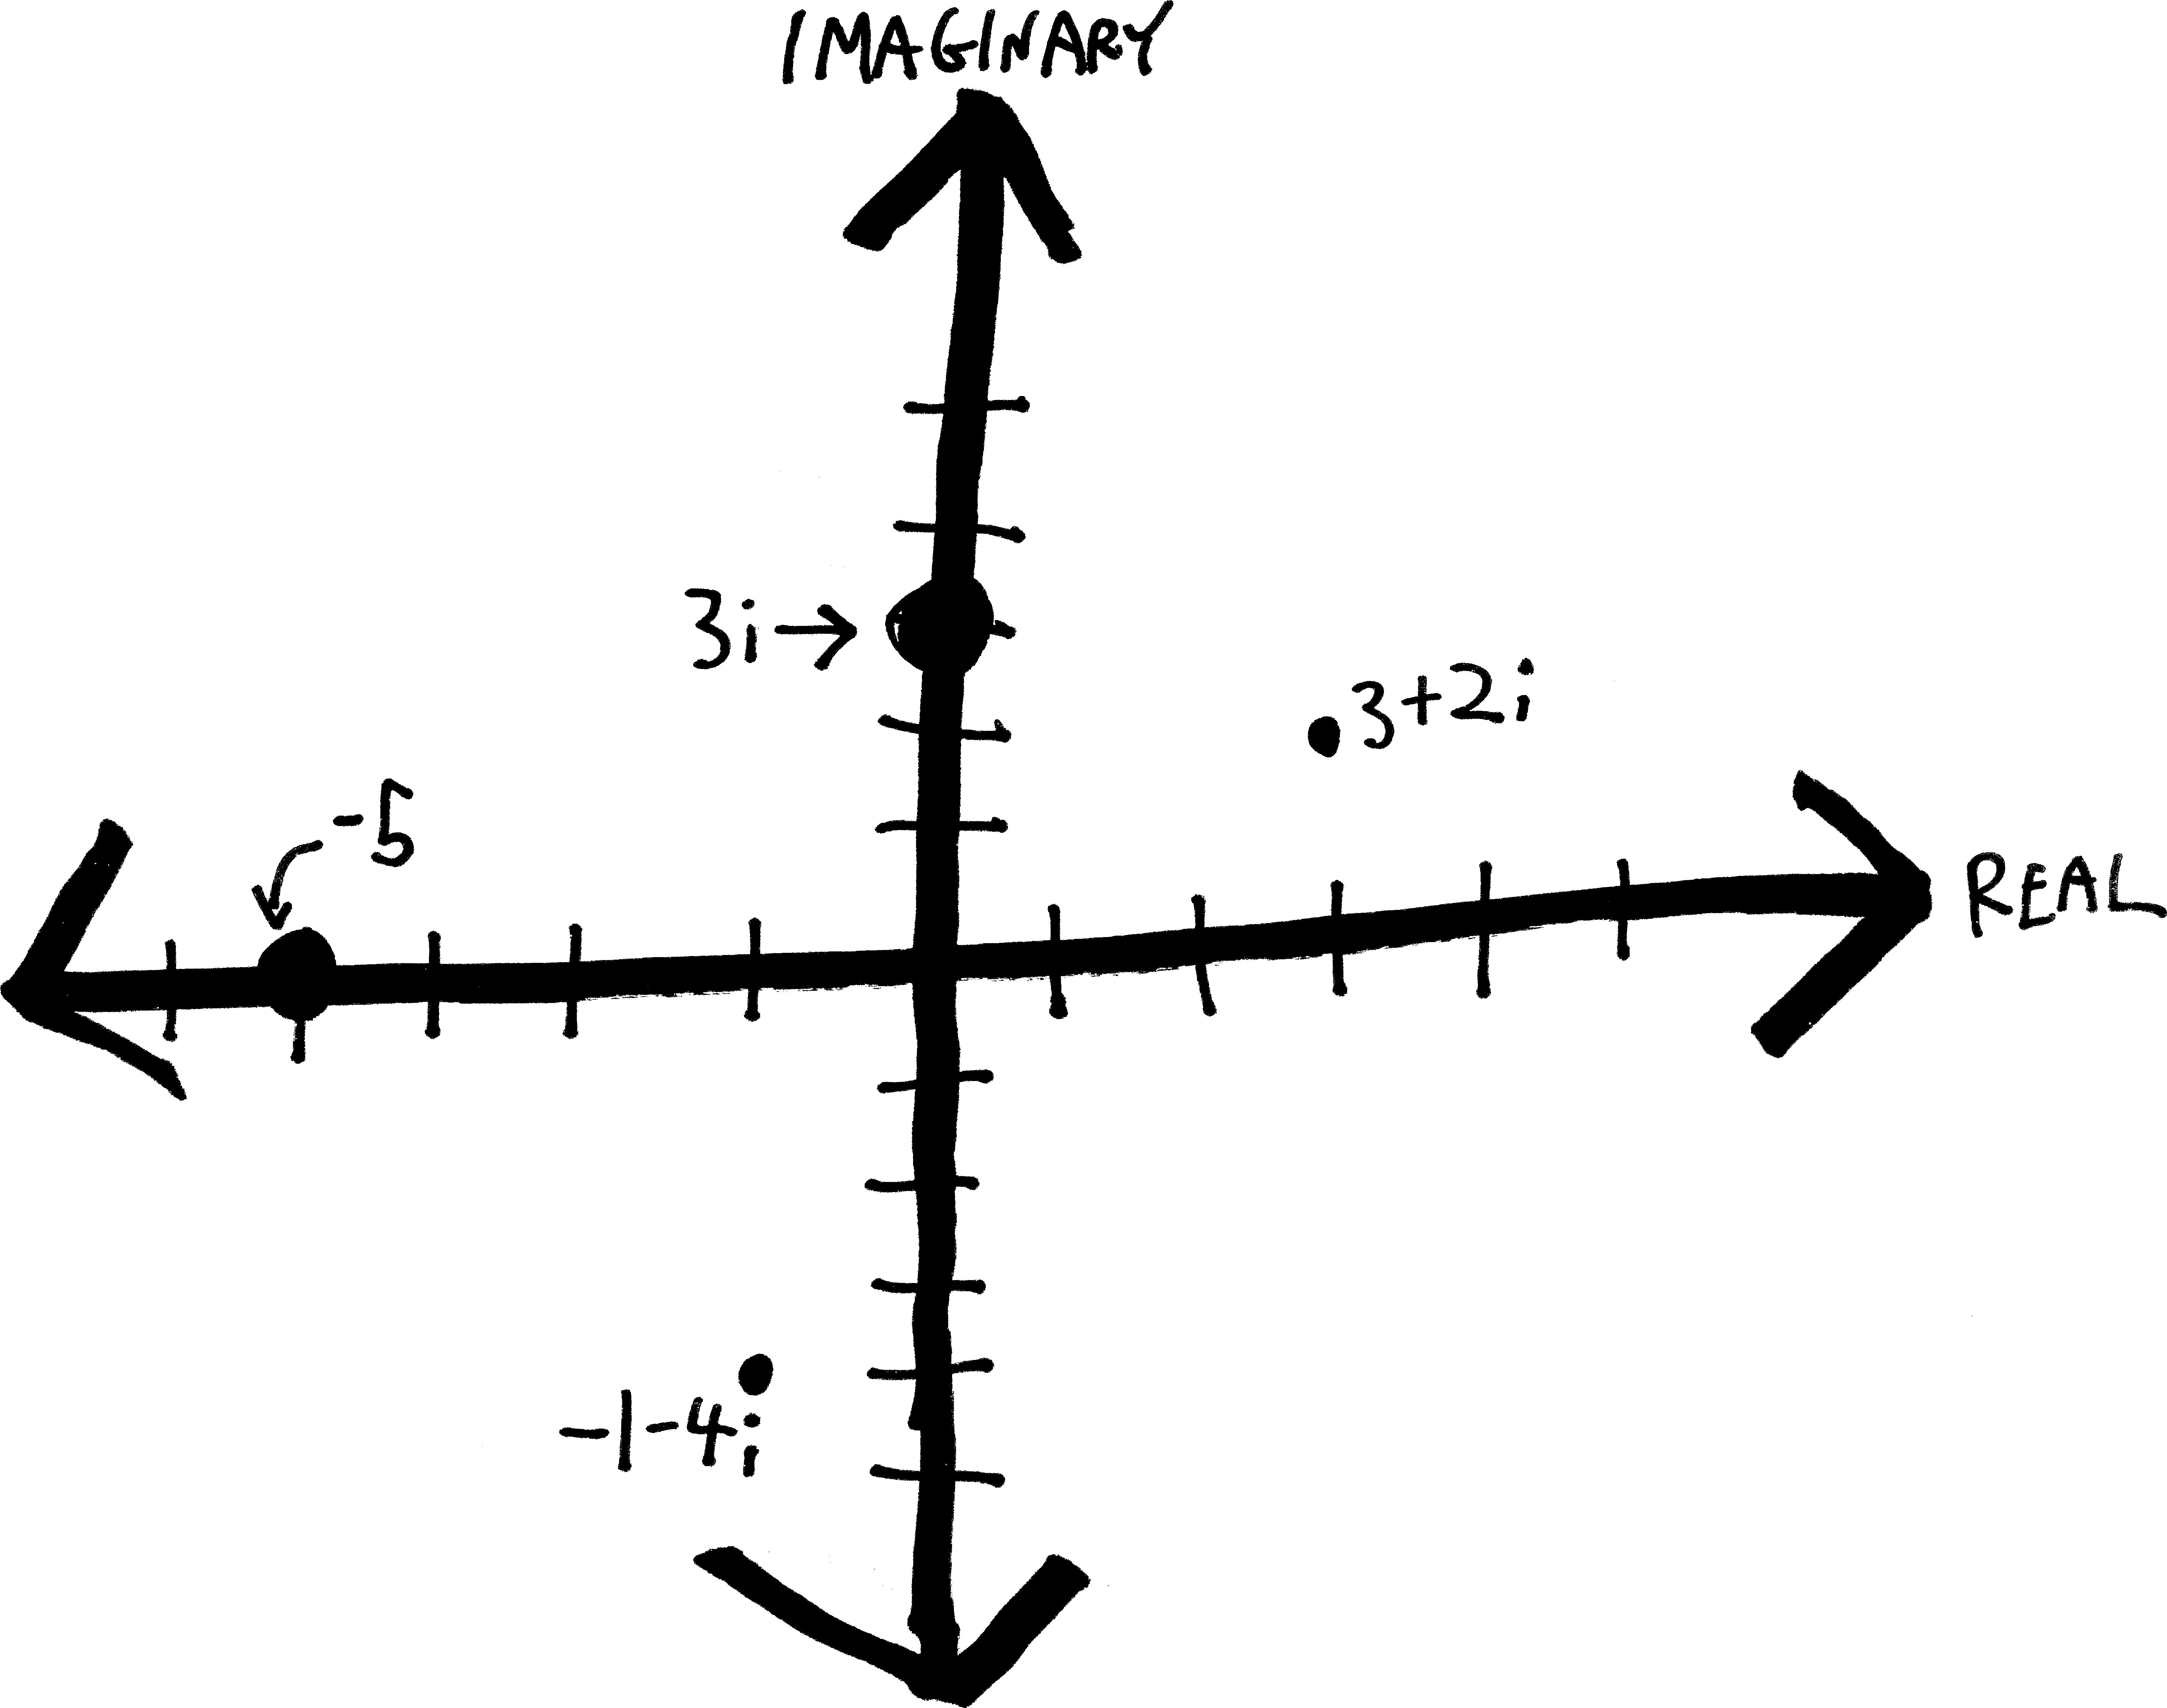
\includegraphics{complex-plane.png}

\hypertarget{some-basic-algebra-with-complex-numbers}{%
\subsection{Some Basic Algebra With Complex
Numbers}\label{some-basic-algebra-with-complex-numbers}}

Suppose we have an equation involving a complex number:

\[4i = z^2 + z\]

We'd like to be able to find what values of \(z\) make this equation
true. Maybe there's one value, maybe there are multiple values, maybe
there are no values. We're pretty good at solving equations with real
numbers! But what about with complex numbers? I guess we could factor
the right-hand side:

\[4i = z(z+1)\]

But that's not very helpful, since the left side is \(4i\), not \(0\),
so it's not as easy as just solving the factors individually.

Here's a better idea. There's a useful trick for solving equations with
complex numbers: every complex number is \emph{made up of two real
numbers}, so \textbf{if we have one equation relating one complex
number, we can turn it into two equations relating two real numbers}.
Let's continue this example so that I can show you what I mean.

We have this complex number \(z\), and we know that any complex number
can be written in the form \(a+bi\), where \(a\) and \(b\) are both real
numbers. So then we can turn this equation about a complex number into
an equation about some real numbers, \(a\) and \(b\):

\[4i = (a+bi)^2 + (a+bi)\]

If we simplify that a bit, we get:

\[
\begin{align*}
4i &= a^2 + 2bi + b^2i^2 +a+bi \\
4i&= a^2 + 2bi - b^2 + a + bi &\text{(because $i^2=-1$)}\\
4i&= a^2 - b^2 + a + 3bi
\end{align*}
\]

Then we've got two complex numbers---one on the left side of the
equation, and one on the right side:

\[
\begin{align*}
0+4i &= \left(a^2 - b^2 + a\right) + 3bi\\ \\
\underbrace{0}_{\text{real part}} + \underbrace{4}_{\text{imaginary part}}\cdot i \quad&=\quad (\underbrace{a^2 - b^2 + a}_{\text{real part}}) +\underbrace{3b}_{\text{imaginary part}}\cdot i
\end{align*}
\]

This looks like one equation with two unknowns---but actually it's
\emph{two} equations! Since these two complex numbers on the left and on
the right are equal, \textbf{their real and imaginary parts must also be
equal}. So then, we can set the imaginary parts equal to each other:

\[4 = 3b\]

\[b = 4/3\]

And we've found \(b\)! We're halfway there to finding the complex number
we're looking for, \(z=a+bi\). Now we just need to find \(a\). So we can
set the real parts equal:

\[0 = a^2 - b^2 + a\]

Since we've found out that \(b=4/3\), we can plug that in:

\[0 = a^2 - \left(\frac{4}{3}\right)^2 - a\]

Looks like we have a quadratic!

\[0 = a^2 + a - \left(\frac{4}{3}\right)^2\]

We can try to factor it, but it turns out to be a mess. Let's use the
quadratic equation:

\[
\begin{align*}
a &= \frac{-1 \pm \sqrt{1^2- 4\cdot1\cdot \left(\frac{4}{3}\right)^2 }}{2} \\
&\vdots \\
&\text{a whole bunch of arithmetic later...} \\
&\vdots \\
&= \frac{-1}{2} \pm\frac{\sqrt{13}}{4} \\
\end{align*}
\]

So we've found what \(a\) can be! There are two possibilities! So we
have:

\[a= \left\{\frac{-1}{2} +\frac{\sqrt{13}}{4} , \quad \frac{-1}{2} -\frac{\sqrt{13}}{4} \right\}\quad\text{and}\quad b=4/3\]

So then there are two possible solutions for \(z\):

\[
\begin{align*}
z =& a+bi \\
= &\left(\frac{-1}{2} +\frac{\sqrt{13}}{4}\right)  \quad+\quad\frac43i ,\\
&\left(\frac{-1}{2} -\frac{\sqrt{13}}{4} \right) \quad+\quad\frac43i 
\end{align*}
\]

Boy, that's a lot of work! Maybe I should have made a simpler example.
Oh well! If you want to verify that those are both solutions, you can
plug them back into the original equation.

\hypertarget{wait-one-more-fun-thing}{%
\subsection{Wait, One More Fun Thing}\label{wait-one-more-fun-thing}}

\(i\) is the square root of negative one---but what if we take \emph{the
square root of \(i\)}?!? Can we even do that?? We saw that cool things
happen when we take powers of \(i\); do cool things happen when we take
roots of \(i\)?

Like with dividing numbers, our first question should be: if we take the
square root of \(i\), do we even still get a complex number? Or will we
get a type of number that's maybe more complex than a complex number? Or
a type of number that's more simple? Or what???

I guess one way we could start to think about this is to realize that
\(i\) is itself a square root, and so maybe we should write that out:

\[\sqrt{i} = \sqrt{\sqrt{-1}} = \left((-1)^{1/2}\right)^{1/2} = (-1)^{1/4} = \sqrt[4]{-1}\]

Hmm. That doesn't seem to tell us a whole lot. Let's try something else.

Let's assume, for a moment, that if we take the square root of \(i\), we
get another complex number as a result. If this complex number has real
part \(a\) and imaginary part \(b\), then we should have:

\[\sqrt{i} = a + bi\]

Or, in other words:

\[i = (a+bi)^2\]

This is something we might be able to do something with! Let's expand
the right side and see what happens. Maybe we'll be able to solve for
\(a\) and \(b\), and thus find the square root of \(i\):

\[
\begin{align*}
i &= (a+bi)^2 \\
 &= a^2 + 2abi + bi^2 \\
 &= a^2 - b^2 + 2abi &\text{because } i^2=-1
 \end{align*}
 \]

But now, we've proven that \(i\) (on the left) must be equal to this
more complicated thing (on the right). We have a complex number on the
left, and a complex number on the right. They're equal. They're the same
number. So then their real and imaginary components must also be equal.
Showing that a bit more explicitly:

\[
\begin{align*}
0 \quad &+ \quad1\cdot i \\
&\,\,|| \\
(a^2 - b^2) \,&+\,\,(2ab)\cdot i
\end{align*}
\]

The real parts and imaginary parts must be equal---so we get two
equations! And we have two unknowns, so we can solve them!

Our first equation, from the real component, is:

\[0 = a^2-b^2\]

So then \(a^2=b^2\), or just that:

\[a = \pm b\]

We need the plus-or-minus, because of course the squaring will destroy
it.

Meanwhile, the other equation (the imaginary component) gives us:

\[2ab = 1\]

Let's plug the stuff from the first equation into this one. If we plug
in \(a=-b\), we get:

\[
\begin{align*}
2(-b)b &= 1 \\
-2b^2 = 1 \\
b = \pm \sqrt{-1/2}
\end{align*}
\]

BUT we know that \(b\) (as well as \(a\) has to be a real number! That's
part of the setup here. Ultimately we're talking about complex numbers,
but we've split our complex number into its components \(a\) and \(b\).
Both of those numbers are real. There's no real number equal to
\(\sqrt{-1/2}\). So this begets no solution. In other words, \(a\) can't
be equal to \(-b\). It can thus only be equal to the other alternative,
\(+b\).

What about if we plug in \(a=+b\)? Then we get:

\[
\begin{align*}
2(b)b &= 1 \\
2b^2 &= 1 \\
b &= \pm 1/\sqrt{2}
\end{align*}
\]

So we've found \(b\)! And we know, from the first equation, that \(a\)
and \(b\) are equal, possibly modulo their sign, except we also found
out that \(a\) can't be negative \(b\). So we have two possibilities:

\[a = b = \frac{1}{\sqrt{2}}\]

\[a = b = \frac{-1}{\sqrt{2}}\]

And then we've done it! We've found the square root of \(i\)!!! We have:

\[\sqrt{i} = \left\{ \frac{1}{\sqrt{2}}+\frac{1}{\sqrt{2}}i \,,\quad \frac{-1}{\sqrt{2}}+\frac{-1}{\sqrt{2}}i \right\}\]

That's so weird! Where does this come from? Is there a better
explanation for why \(\sqrt{i}\) is this weird number with fractions and
\(\sqrt{2}\)? What if we want to find not just the square root of \(i\),
but the cube root? or the quartic root? or the quintic root? or the
\(n\)'th root? Do we have to do all this nasty, nasty algebra (which, no
doubt, will just get worse)? By the way, can we graph these two
solutions? What happens? Where are they on the complex plane?
Incidentally, doesn't \(1/\sqrt{2}\) seem familiar?? Have we seen that
anywhere else recently??

If you don't believe that that really is the square root of \(i\)---if
you think our procedure, what with its assumptions, equating real and
imaginary components, etc., was a bunch of malarkey---try squaring one
(or both) of these. What happens?

\[\left(\frac{1}{\sqrt{2}}+\frac{1}{\sqrt{2}}i\right)^2 = \hspace{3in} \]

\[\left(\frac{-1}{\sqrt{2}}+\frac{-1}{\sqrt{2}}i\right)^2 = \hspace{3in}\]

Incidentally, we've answered our question about whether the square root
of \(i\) is itself a complex number---it is! We can write it in the form
\(a+bi\), so it is indeed complex.

COMPLEX NUMBERS ARE SO WEIRD, eh???

\vspace{3pc}

\centerline**

\Large Problems\footnote{Many/most of these problems, especially the hard ones are stolen from the Art of Problem Solving's *Intermediate Algebra}
text (which in turn stole many of its problems from various math
contests!). \}\}

\vspace{1pc}

\noindent For each of the following pairs of complex numbers \(z\) and
\(w\):

\begin{enumerate}[label=\alph*.]
  \setlength{\itemsep}{1pt}
  \setlength{\parskip}{0pt}
  \setlength{\parsep}{0pt}
\item Plot $z$ and $w$ on the complex plane.
\item Perform the following arithmetic operations, and plot the result (clearly labelled) on the same complex plane (i.e., the same axes):
\begin{enumerate}[label=(\roman*)]
\item $z+w$
\item $z-w$
\item $z\cdot w$
\item $z/w$
\end{enumerate}
\item Also, find $\overline{z}$ and $\overline{w}$. Draw them on your (hopefully not too messy? maybe you could use colors?) graph, too\footnote{These problems, though, I (mostly) randomly generated with three lines of Python!}
\end{enumerate}

\begin{multicols}{3}
\setlength{\columnseprule}{.5pt}
\begin{problems}
\item $z=0$; $w=0$
\item $z=1$, $w=0$
\item $z=5$; $w=3$
\item $z=1$; $w=i$
\item $z=3+4i$; $w=12-5i$
\item $z=2i$; $w=7-2i$
\item $z=2-5i$; $z=-3+i$
\item $z=1$; $w=2+i$
\item $z=3+2i$; $w=4$
\item $z=5-3i$; $w=2-i$
\item $z=1+2i$; $w=-1+4i$
\item $z=2-i$; $w=7+9i$
\item $z=11+4i$; $w=2+15i$
\item $z=10-5i$; $w=3+10i$
\item $z=9+13i$; $w=5+9i$
\item $z=2+i$; $w=2+15i$
\item $z=15-5i$; $w=-2-5i$
\item $z=14+10i$; $w=15+7i$
\item $z=7+12i$; $w=13+12i$
\item $z=11+2i$; $w=-4+14i$
\item $z=11+i$; $w=6+3i$
\item $z=8+13i$; $w=9+2i$
\item $z=8+10i$; $w=10+10i$
\item $z=-5+5i$; $w=7+12i$
\item $z=4+9i$; $w=3$
\item $z=7+8i$; $w=14+14i$
\item $z=12+-3i$; $w=12+8i$
\item $z=-2+i$; $w=-1+8i$
\item $z=-4$; $w=12-3i$
\item $z=8+8i$; $w=3+4i$
\item $z=2+6i$; $w=15+10i$
\item $z=1+15i$; $w=8+6i$
\end{problems}
\end{multicols}

\noindent Let's do some algebra with complex numbers! Solve each of the
following equations for \(z\). (Since we know that we can represent any
complex number as its real part plus its imaginary part times \(i\), it
might be a good idea to rewrite \(z\) like that! Or it might not.)

\begin{multicols}{2}
\setlength{\columnseprule}{.5pt}
\begin{problems}
\setcounter{enumi}{32}
\item $z+5 = 8+2i$
\item $z-i = 12$
\item $z+9+8i = 6$
\item $5z = 3i$
\item $7z = 2+4i$
\item $z^2 + 5z + 1 = 0$
\item $z^2 + 9z + 15 = 0$
\item $(6+3i)^2=4i-30z$
\item $\displaystyle \frac{2z-3i}{z+4} = -5+i$
\item $z^2+81 = 0$
\item $\displaystyle \frac{z+3i}{z-3} = 2$
\item $\displaystyle \frac{1+2i}{3z} = 4+5i$
\item $\displaystyle 3z+\frac{z}{1+i} = 10-4i$
\item $z + 2\overline{z} = 6-4i$
\item $z^2 = 21 - 20i$
\item $\displaystyle \frac{z-2}{z+1} =3i $
\item $z^2 + 5z = -6$
\end{problems}
\end{multicols}

\vspace{1pc}

\noindent More algebra! Solve for \(x\) and \(y\), where \(x\) and \(y\)
are both real numbers! (It might help to remember that two complex
numbers are equal if and only if their real and imaginary components are
equal---so from an equation relating two complex numbers, we can
actually get \emph{two\} equations relating }two each\} real numbers.)

\begin{multicols}{2}
\setlength{\columnseprule}{.5pt}
\begin{problems}
\setcounter{enumi}{49}
\item $(x+yi)(2-i)=-i$
\item $(x+2i)(1-i) = 5+yi$
\item $(x-2)(3yi+5i) = 4+x-i$
\item $3x + (3x - y)i = 4 - 6i$ 
\item $2y+xi= 4+x-i$
\item $2x+3yi = -x-6i$
\item $(x+yi)(2-i)=8+i)$
\item $x^2+xi=4-2i$
\item $(3+2i)(x+yi)=-i$
\item $2(x+yi)=x-yi$
\item $(x+i)(3-iy)=1+13i$
\item $(x+2i)(y-i)=-4-7i$
\item $(x+yi)(2+i) = 2x- (y+1)i$
\end{problems}
\end{multicols}

\vspace{1pc}

\begin{problems}
\setcounter{enumi}{62}
\item Simplify: $\displaystyle \frac{a+bi}{b-ai}$ (where $a$ and $b$ are real numbers)
\item Simplify: $\displaystyle \left(2i^{18}-3\right)\frac{2+6i}{4+i}$
\item Find all values of $k$ such that $(3+2i)(3+ki)$ is a real number.
\item Simplify $\displaystyle \frac{z+\overline{z}}{2}$. Is it something cool?!? (To be clear about what I mean by ``simplify,'' I mean, if we write $z$ as $z=a+bi$, and then simplify things, what's the new complex number we get?)
\item Likewise, simplify $\displaystyle \frac{z-\overline{z}}{2i}$. What happens?!?
\item What is $(i-i^{-1})^{-1}$? 
\item Simplify $\displaystyle \frac{1}{1+\frac{1}{1-\frac{1}{1+i}}}$
\item Simplify:
\begin{enumerate}
\item $\displaystyle \sum_{k=0}^{k=\infty}i^k$ \smallskip
\item $i+i^2+i^3+i^4$ \smallskip
\item $\displaystyle \sum_{k=1}^{k=2000}i^k$ \smallskip
\item $\displaystyle \sum_{k=1}^{k=347}i^k$ \smallskip
\item $\displaystyle \sum_{k=0}^{k=100}i^{2k+1}$ \smallskip
\item $\displaystyle \sum_{k=0}^{k=1000}i^{8k+2}$\smallskip
\end{enumerate}

\item We didn't answer our original question about dividing complex numbers. Namely, when we divide two complex numbers, is the result *always} also a complex number? Or is the result potentially sometimes a weirder and more bizarre form of number? 
\begin{enumerate}
\item Figure it out! Here's my suggestion: suppose we have two complex numbers:
$$z_1 = a+bi$$
$$z_2=c+di$$
Because $a$, $b$, $c$, and $d$ are real numbers, and can be *any} real number, these two complex numbers are in fact *any} and *every complex number!} Then, try dividing $z_1$ and $z_2$ (in either order). As usual when dividing complex numbers, you should eventually get something like:
$$\frac{a+bi}{c+di} = (\text{a whole buncha stuff}) +(\text{a whole bunch more stuff})\cdot i$$
In order for $\frac{a+bi}{c+di}$ to be a complex number, its real and imaginary components (i.e., ``a whole buncha stuff'' and ``a whole bunch more stuff'') must both be real numbers. Are they? Why, or why not?

\item Now that you've worked that out, you have a formula that tells you how to divide complex numbers. Which would you rather do (when it comes time for you to divide two complex numbers): memorize the formula and then plug things in, or memorize the ``multiply by the conjugate of the denominator'' procedure? (There's not a right answer!)
\end{enumerate}

\item Complex conjugates are cool! Let's prove some stuff about them:
\begin{enumerate}
\item Prove that any complex number times its conjugate is a real number. (Actually, we did this already.)
\item Prove that we can split complex conjugates up along addition. In other words, show that for any two complex numbers $z$ and $w$, we have $\overline{z+w} = \overline{z}+\overline{w}$
\item Prove that we can split complex numbers up along multiplication, in other words, show that for any two complex numbers $z$ and $w$, we have $\overline{z\cdot w} = \overline{z}\cdot\overline{w}$
\item Can we split complex conjugates up along subtraction? Prove or disprove. (Note that to disprove, all you need to do is find a counterexample!)
\item Can we split complex conjugates up along division? Prove or disprove.
\end{enumerate}
\item More questions about complex conjugates!
\begin{enumerate}
\item What's the conjugate of a conjugate? In other words, for some complex number $z$, simplify $\overline{\overline{z}}$.
\item When (if ever) is $\overline{z}=z$?
\item When (if ever) is $\overline{z} = -z$?
\end{enumerate}
\item Let $w$ and $z$ be complex numbers.
\begin{enumerate}
\item Show that $w\overline{z} + \overline{w}z$ is always real.
\item Show that $w\overline{z} - \overline{w}z$ is always imaginary.
\end{enumerate}
\end{problems}

\textbackslash end\{document\}

\end{document}
